\pdfoutput=1
\pdfcompresslevel=9
\pdfinfo
{
    /Author ()
    /Title ()
    /Subject ()
    /Keywords ()
}
\documentclass[a4paper,onecolumn,oneside,12pt]{mwrep}


\usepackage{url}
\usepackage{times}
\usepackage{polski}
\usepackage[utf8]{inputenc}
\usepackage[T1]{fontenc}
\usepackage{setspace}
\usepackage{graphicx}
\usepackage{pgfplots}
\usetikzlibrary{pgfplots.groupplots}
\usepackage{listings}
\lstset{basicstyle=\footnotesize\ttfamily,columns=fullflexible}
\usepackage{tikz} 

\hyphenpenalty=10000        % nie dziel wyrazów zbyt często
\clubpenalty=10000          % kara za sierotki
\widowpenalty=10000         % nie pozostawiaj wdów
\brokenpenalty=10000        % nie dziel wyrazów między stronami
\exhyphenpenalty=999999     % nie dziel słów z myślnikiem
\righthyphenmin=3           % dziel minimum 3 litery

\tolerance=4500
\pretolerance=250
\hfuzz=1.5pt
\hbadness=1450

\sloppy                     % umacnia pozycję prawego marginesu

\setlength{\textwidth}{\paperwidth}
\addtolength{\textwidth}{-5cm}
\setlength{\textheight}{\paperheight}
\addtolength{\textheight}{-5cm}
\setlength{\oddsidemargin}{0cm}
\setlength{\evensidemargin}{0cm}
\topmargin -1.25cm
\footskip 1.4cm

\linespread{1.3}

\begin{document}

\begin{titlepage}
    \begin{center}
        \fontsize{14pt}{12px}\selectfont
        \textbf{POLITECHNIKA WARSZAWSKA} \\
        WYDZIAŁ ELEKTRYCZNY \\
        INSTYTUT STEROWANIA I ELEKTRONIKI PRZEMYSŁOWEJ

        \vspace*{.6\baselineskip}

        \fontseries{b}\fontsize{12pt}{10pt}\selectfont
        PRACA DYPLOMOWA MAGISTERSKA \\
        na kierunku INFORMATYKA \\
        specjalność: inżynieria oprogramowania
    \end{center}

    \begin{flushleft}
        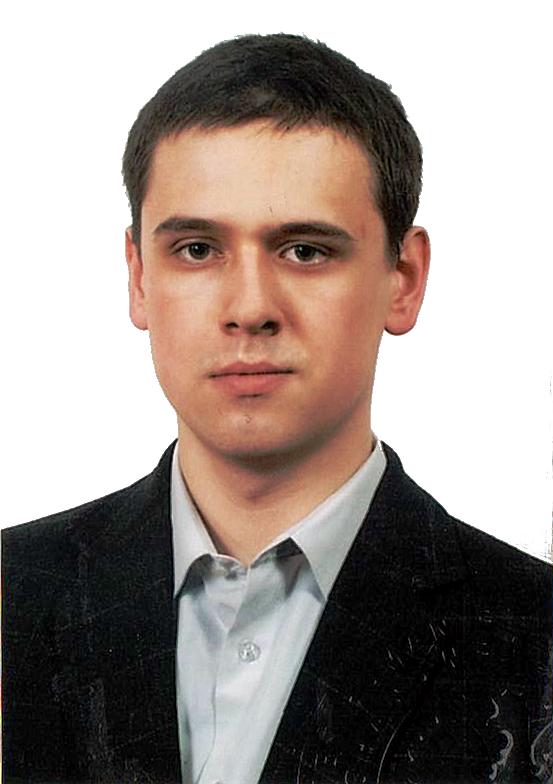
\includegraphics[width=4cm]{img/zdjecie_dyplo.png} \\
        \fontsize{14pt}{12px}\selectfont
        Jakub SAŁKOWSKI \\
        \fontseries{b}\fontsize{12pt}{10pt}\selectfont
        Nr albumu: 248418
    \end{flushleft}

    \begin{flushright}
        \begin{minipage}{0.3\textwidth}
            \fontsize{12pt}{10pt}\selectfont
            Rok akad.: 20013/2014 \\		
            \fontsize{10pt}{8pt}\selectfont
            Warszawa, \textit{2013.05.12}
        \end{minipage}
    \end{flushright}

    \vspace*{1\baselineskip}

    \begin{center}
        \fontseries{b}\fontsize{14pt}{12pt}\selectfont
        PROJEKT I~REALIZACJA APLIKACJI ODCZYTUJĄCEJ NUMERY
        AUTOBUSÓW NA URZĄDZENIA MOBILNE Z SYSTEMEM ANDROID
    \end{center}

    \vspace*{1\baselineskip}

    \begin{flushleft}
        \fontseries{b}\fontsize{12pt}{10pt}\selectfont
        Zakres pracy:
        \fontseries{m}\fontshape{it}\selectfont
        \begin{enumerate}
            \item Wprowadzenie i~sformułowanie celu pracy
            \item Przegląd metod detekcji
                i~identyfikacji obiektów w obrazach
            \item Przygotowanie środowiska wspomagającego
                implementację i~weryfikację algorytmów
            \item Analiza porównawcza wybranych
                metod detekcji i~identyfikacji obiektów w~obrazach
            \item Implementacja i~weryfikacja najbardziej efektywnego algorytmu
                na kilku urządzeniach z~systemem Android
            \item Wnioski i~podsumowanie
        \end{enumerate}
        \fontshape{n}\fontseries{b}
        \fontsize{12pt}{10pt}\selectfont

        \vspace*{1\baselineskip}

        Kierujący pracą: \textit{dr inż. Witold Czajewski} \\

        \vspace*{4\baselineskip}

        \fontseries{m}\selectfont
        Termin złożenia pracy: \textit{2014.09.15} \\
        \fontsize{10pt}{8pt}\selectfont
        Praca wykonana i obroniona pozostaje \\
        własnością Instytutu, Katedry i nie będzie \\
        zwrócona wykonawcy.
    \end{flushleft}
\end{titlepage}


\tableofcontents


% streszczenie
\begin{center}
	\textbf{Streszczenie}
\end{center}

W~ramach pracy wykonano projekt oraz implementację aplikacji możliwej do zainstalowania 
i~uruchomienia
na urządzeniu mobilnym z~systemem Android. Głównym i~jedynym 
zadaniem wytworzonego oprogramowania
było odczytywanie numeru linii z~frontu nadjeżdżającego autobusu.
Zgodnie z~architekturą, program po uruchomieniu na telefonie
wchodził w~tryb pobierania klatek obrazu z~aparatu urządzenia. 
Po pobraniu zadanej z~góry liczby klatek z~wystąpieniem frontu
autobusu następował odczyt.

W~pierwszej części pracy zamieszczono przegląd narzędzi, algorytmów,
bibliotek i~struktur ramowych służących do wykrywania obiektów w~scenach
oraz ich identyfikacji - rozpoznawania. Przygotowany w~ten sposób
zbiór narzędzi i~technik wykorzystano w~celu wyłonienia tych najbardziej
adekwatnych w~danym zagadnieniu. Główne kryteria przy doborze to m.in:
skuteczność, łatwość implementacji, dostępna dokumentacja oraz możliwość
konfiguracji.

Następnie zamieszczono opis przeprowadzonych eksperymentów
mających na celu wyłonienie najpewniejszych rozwiązań, które
zostały wykorzystane do skonstruowania ostatecznej implementacji.
W~pracy zawarty został też opis prób podjętych w~celu automatyzacji
procesu przygotowywania oraz weryfikacji powstających narzędzi 
i~programów.

Praca dokumentuje i~systematyzuje zastosowane pomysły i~metody.
Część okazała się nietrafiona, co skutecznie uniemożliwiło ich
wykorzystanie w~rozwiązaniu docelowym. W~wyniku
bardzo licznych eksperymentów udało się wyłonić zbiór 
narzędzi, dzięki którym implementacja była wykonalna.

Wykonane testy skuteczności pomogły w~określeniu niezawodności,
a~przez to przydatności wykonanej aplikacji. Na szczęście
modułowa budowa programu umożliwiała doskonalenie oraz
wymianę poszczególnych jej elementów. Ścieżki rozwoju
i~możliwości usprawnień zostały przedstawione w~ostatniej
części pracy.


\vspace*{\baselineskip}

\noindent\textbf{Słowa kluczowe:} \textit{Android, OpenCV, Tesseract,
widzenie komputerowe, detektory kaskadowe, 
wykrywanie obiektów, rozpoznawanie obiektów,
OCR, odczytywanie numeru autobusu.}

\vspace*{2\baselineskip}
\newpage

\begin{center}
	\textbf{Abstract}
\end{center}

This paper describes process of design and implementation
of an Android application which could help or even replace 
humans at reading city bus line numbers from the front 
part of the aproaching vihicle. Initial design assumed
that first prototype application would have very limited functionality.
Just after first lunch, program would try to find bus front 
in each frame taken from device camera. After first positive
check, fixed number of frame shall be taken and processed
in case of bus front identification and localization, number
localization and filally recognition of digits in the identified number.

First described activity was the review of available tools, algorythms,
libraries and frameworks which could be helpful in object
detection and recognition in natural scenes. Preapred set of
tools and techniques was reviewed to choose most usefull ones
for each problem. Main criteria were: efficiency and effectiveness,
ease of implementation,
available documentation and possible configuraion.

In next chapter description of conducted experiments was made.
Performed tests were supposed to help in finding 
best suited algorithms and implementation of those
algorithms according to the problem which shall be solved.
After many hours and days spent on preparing and
executing tests the fixed set of tools was chosen 
to make final implementation. At this stage it was 
certain that application was doable.

Extensive test results allowed to determine the effectiveness
and hence the usefulness of proposed applicaiton.
Focus put on modularity led to the fact that implemented
software was easly extendable. Every step of algorithm 
could be improved separately or even raplaced whith completely
different one. Paths of development and improvement
were described in the last chapter.

\vspace*{\baselineskip}
\noindent\textbf{Keywords:} \textit{Android, OpenCV, Tesseract,
	cumputer vision, cascade detectors, 
	object detection, object recognition,
	OCR, city bus number reading.}

\setcounter{page}{2}


\chapter{Wprowadzenie}

Widzenie maszynowe jest jedną z~najprężniej rozwijających się
dziedzin z~pogranicza algorytmiki, optymalizacji, przetwarzania obrazów,
przetwarzania sygnałów, statystyki oraz szeroko pojętej sztucznej
inteligencji, jeżeli chodzi o~zagadnienia informatyczne w~ostatnich
latach. Sporządzenie definicji widzenia komputerowego jest niezmiernie
trudne. Głównie z~powodu wspomnianej interdyscyplinarności
jaką niesie ze sobą omawiany termin. Klasyczne, jednozdaniowe
definicje przedstawiają w~zwięzły sposób ogólny zarys koncepcji
jaka kryje się za sformułowaniami określanymi mianem wizji komputerowej.
Wysoki poziom abstrakcji oraz zwięzłość formy zmuszają do pominięcia
wielu istotnych aspektów, które nienaświetlone mogą w~poważny sposób
zaburzyć wyobrażenie o~tym niezmiernie interesującym 
obszarze nauki i~techniki.  
Poniżej przedstawiono kilka definicji wprowadzonych na przestrzeni
kilkunastu ostatnich lat. 

DEFINICJA 1 \cite{ShapiroStockman200102}:

,,Zadaniem wizji komputerowej jest podejmowanie 
decyzji na temat rzeczywistych (fizycznych) obiektów
oraz scen na podstawie obrazów.''

W~komentarzu do zaprezentowanej definicji wprowadzony został
cel pośredni. Aby podjęcie decyzji na temat rzeczywistych obiektów
było możliwe, niemal zawsze niezbędne jest sporządzenie ich modelu lub 
opisu na podstawie posiadanych zdjęć. Zgodnie z~powyższym,
równolegle do poprzedniej definicji, zaproponowana została druga, mniej
abstrakcyjną wersja, którą umieszczono poniżej.

DEFINICJA 2 \cite{ShapiroStockman200102}:

,,Zadaniem wizji komputerowej jest sporządzanie
opisów scen rzeczywistych na podstawie obrazów.''

Jest to pierwsza próba ograniczenia danych wyjściowych jakich należałoby
oczekiwać po uruchomieniu procesu określanego mianem wizji komputerowej.

Następna definicja jest kolejną próbą
podjętą w~kierunku maksymalnego uproszczenia i~zawężenia
przeciwdziedziny widzenia komputerowego. Nie ulega raczej wątpliwości,
że danymi wejściowymi procesu są obrazy lub sekwencje obrazów.
W~tym kontekście następne zdanie definiuje produkt omawianego zagadnienia.

DEFINICJA 3 (na podstawie \cite{morris2004computer}):

,,Wizja komputerowa obejmuje swym zakresem wydobywanie
danych numerycznych z~obrazów.''

Tak jak przetwarzanie obrazów określa działania na obrazach wynikiem
których są obrazy o~zmienionych właściwościach w~porównaniu do obrazów
wejściowych, tak wynikiem widzenia komputerowego są dane wydobywane
z~obrazów. Dane wyłuskane w~ten sposób mogą zostać wykorzystane
na wiele sposobów:
\begin{itemize}
    \item prezentując wartość samą w~sobie, np.: odczyt tekstu
        z~zeskanowanych dokumentów (OCR),
    \item określając współrzędne elementów sceny, w~kontekście OCR 
        i~odczytywania tekstu z~dokumentów dane tego typu
        wykorzystywane są do zachowania struktury dokumentu, tabel,
        obrazów itp.
    \item do uwierzytelniania na podstawie danych biometrycznych - 
        rozpoznawanie i~identyfikacja siatkówki oka,
    \item do budowania modeli trójwymiarowych obiektów na podstawie 
        sekwencji obrazów, itp.
\end{itemize}

Jak łatwo zauważyć widzenie komputerowe to niezwykle pojemny termin.
Interdyscyplinarność czyni próbę wymienienia zagadnień z~nim związanych,
bez pominięcia jakiejś istotnej gałęzi, niemal niemożliwą. 
Złożoność i~rozległość zakresu jaki wiąże się
z~tym zagadnieniem zilustrowano na rys. \ref{fig:int_cv_inter_discip}.

\begin{figure}[!h]
    \centering
    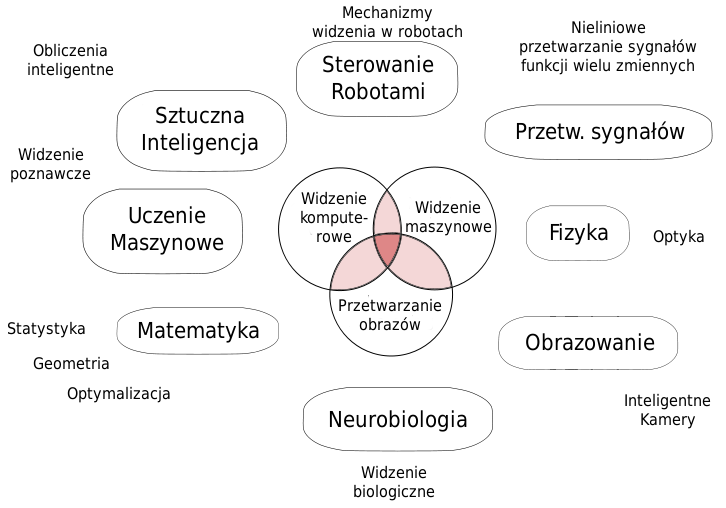
\includegraphics[width=0.9\textwidth]{img/int_cv_inter_discip}
    \caption{Powiązanie wizji komputerowej z~innymi dziedzinami 
        (na podstawie \cite{wiki:computervision})}
    \label{fig:int_cv_inter_discip}
\end{figure}

Narodziny widzenia maszynowego miały
miejsce na początku drugiej połowy ubiegłego wieku.
W~latach pięćdziesiątych wdrożone zostały dwie implementacje 
pierwszego komercyjnego systemu OCR (\textit{ang. Optical Character 
Recognition}). Pierwszym klientem było wydawnictwo Reader's Digest,
gdzie system wykorzystywano do automatycznego odczytywania adresów
z~przesyłek wysyłanych do czytelników w~celu ich sortowania.
Drugim klientem komercyjnego systemu OCR 
była firma Standard Oil Company. Rozwiązanie
służyło odczytywaniu danych z~kart kredytowych w~celach 
rozliczeniowych \cite{WEB:ocrhistory}.

Obecnie istnieje wiele narzędzi do odczytywania tekstu z~zeskanowanych
dokumentów. Najlepsze rozwiązanie dostępne na rynku
można nabyć za cenę zbliżoną do tej w~jakiej oferowany jest
popularny pakiet oprogramowania biurowego.

Według innego opracowania \cite{web:huangcvevolution}
początki widzenia komputerowego są związane z~nazwiskiem Larrego
Robertsa. On to przez swoją pracę doktorską na temat możliwości
wyłuskania trójwymiarowych współrzędnych brył geometrycznych
z~dwuwymiarowych widoków perspektywicznych został okrzyknięty
,,ojcem'' wizji komputerowej. Praca została złożona i~obroniona 
w~latach 60 na uczelni MIT \cite{books/garland/Roberts63}.

Ważnym wydarzeniem z~perspektywy niniejszej pracy dyplomowej była
pierwsza implementacja algorytmu wykrywającego wystąpienie twarzy
w~obrazie w~czasie rzeczywistym.
Na początku obecnego stulecia opracowano oraz zaimplementowano algorytm
\cite{DBLP:conf/cvpr/ViolaJ01}, który uruchomiony na komputerze 
z~procesorem Intel Pentium III 700 MHz był w~stanie przeszukiwać obrazy
pod kątem wystąpienia twarzy w~tempie 15 klatek na sekundę.
Rozdzielczość obrazów wejściowych była równa 384 na 288 pikseli.
Dzisiaj, ze względu na moc obliczeniową urządzeń mobilnych, algorytm ten 
bez trudu można uruchomić
na telefonie lub aparacie fotograficznym. 
Ponadto uzyskane wyniki przekraczają wspomniane 15  na sekundę
przy jednoczesnym wykorzystaniu obrazów wejściowych w~znacznie
większej rozdzielczości: 720p czy nawet 1080p.
Jedną z~bardziej 
popularnych funkcjonalności opartych na wspomnianym rozwiązaniu 
jest wykorzystywany od kilku lat system zwalniania migawki w~aparatach
cyfrowych.
Zdjęcie wykonywane jest
po wykryciu twarzy w~kadrze zawierającej określony grymas, na przykład
uśmiech.

Moc obliczeniowa współczesnych smartfonów pozwala na uruchomienie
znacznie bardziej skomplikowanych algorytmów. Najnowsze jednostki,
wyposażone w~procesory cztero- i~ośmiordzeniowe można nabyć
w~cenie już kilkuset złotych. Dodatkowo mnogość dostępnych bibliotek 
sprawia, że głównym ograniczeniem przy projektowaniu i~implementacji
rozwiązań z~dziedziny widzenia komputerowego jest już niemal
tylko wyobraźnia. Co prawda, utrudnieniem może być słabej jakości
kamera dostępna w~urządzeniu, jednak ograniczenie to obowiązuje
tylko podczas implementacji algorytmów precyzyjnej lokalizacji
i~rozpoznawania obiektów na podstawie danych z~aparatu.

Jednym z~popularniejszych zastosowań widzenia komputerowego w~telefonach
jest odczytywanie kodów QR. Jest to często stosowana technika
np. w~muzeach. Aplikacje udostępniane przez placówki 
umożliwiają uzyskanie szczegółowych opisów eksponatów na
podstawie zamieszczonych obok nich kodów. Zwiedzający mogą w~ten sposób 
skorzystać z~towarzystwa wirtualnego przewodnika. 

Osobną grupę aplikacji stanowią programy napisane z~myślą 
o~niewidomych. W~skład zbioru wchodzą między innymi aplikacje
do rozpoznawania banknotów, obiektów na podstawie
naklejonych kodów QR, odczytywania napisów itp.
Zasadnym wydaje się więc istnienie aplikacji odczytującej numer 
autobusu właśnie w~kontekście wykorzystania przez osoby niewidome lub
niedowidzące. 

Celem niniejszej pracy jest przygotowanie działającej implementacji
algorytmu odczytującego numer zawarty we froncie nadjeżdżającego
autobusu na urządzeniu mobilnym z~systemem Android.
Do osiągnięcia ostatecznego celu niezbędna jest
realizacja następujących celów pośrednich:

\begin{itemize}
    \item przygotowanie
oraz weryfikacja algorytmu detekcji frontów autobusów w~scenie,
    \item lokalizacja numeru linii we froncie autobusu,
    \item rozpoznanie poszczególnych cyfr zawartych
        w~zlokalizowanym fragmencie frontu - odczytanie numeru. 
\end{itemize}

\begin{figure}[!h]
    \centering
    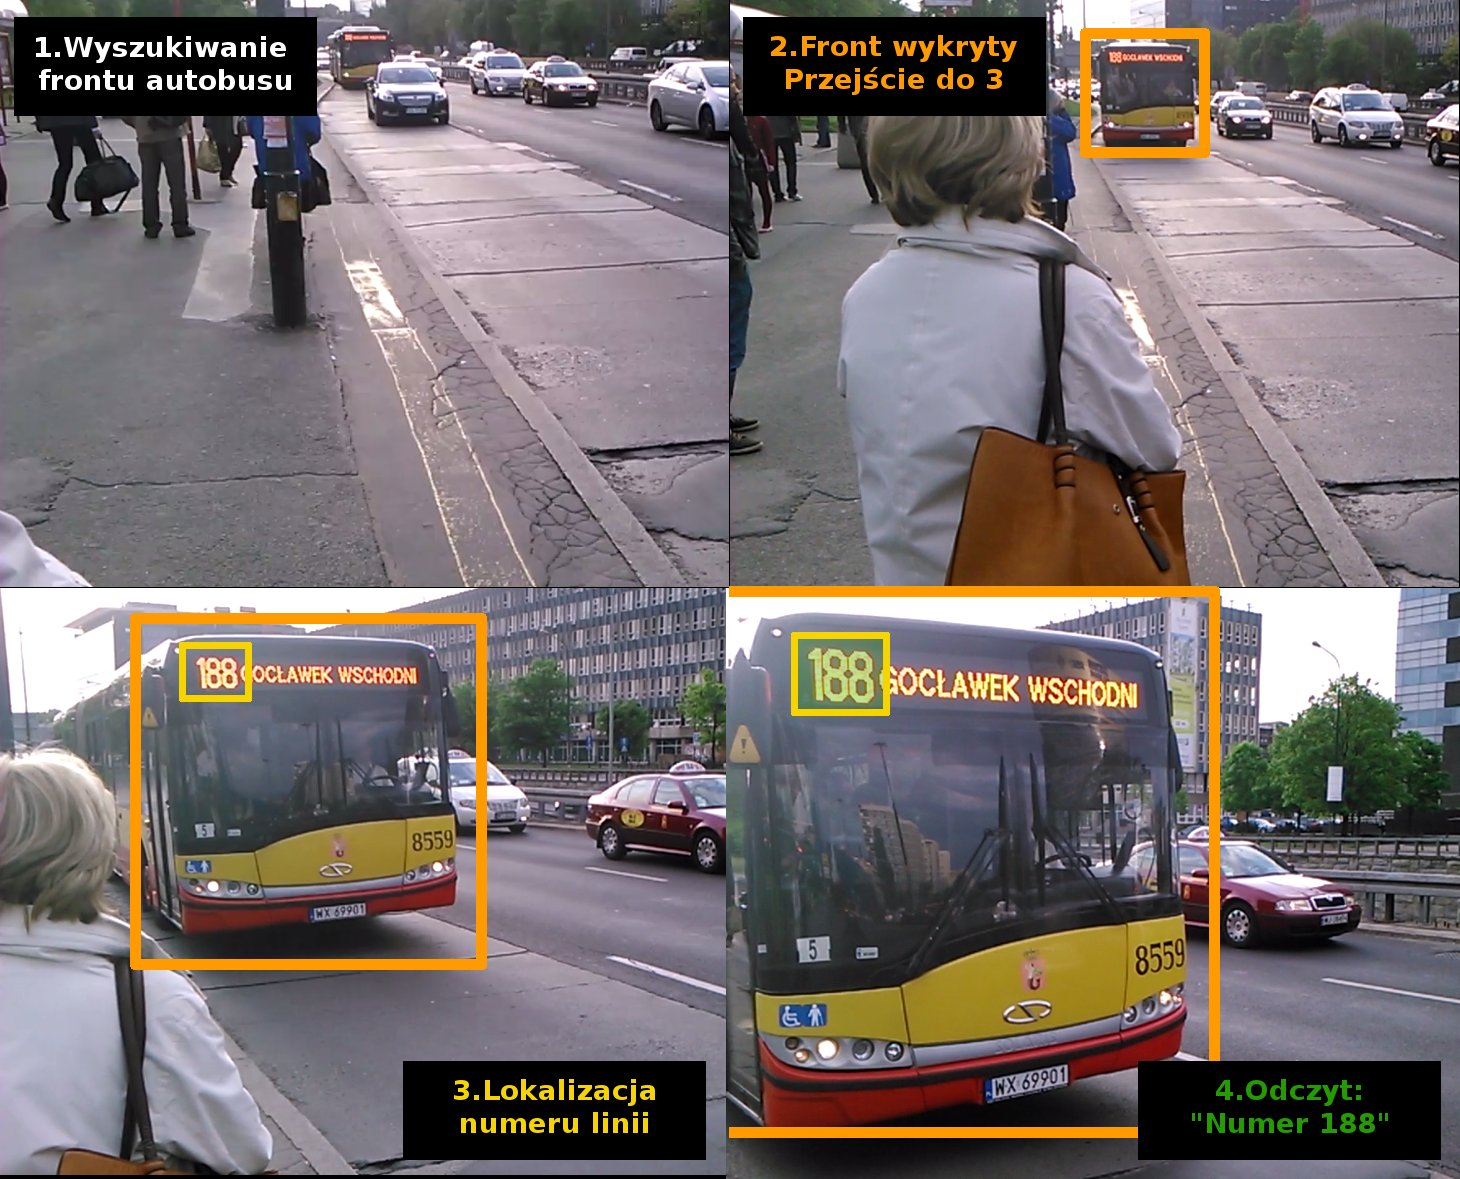
\includegraphics[width=0.9\textwidth]{img/int_use_case_sequence}
    \caption{Diagram przedstawiający przypadek użycia proponowanej aplikacji}
    \label{fig:int_use_case_diag}
\end{figure}

Elementem dodatkowym, nadającym sens całemu rozwiązaniu w~kontekście
wykorzystania aplikacji przez osoby niewidome i~niedowidzące,
byłoby wykorzystanie syntezatora tekstu na mowę dla 
odczytanego przez algorytm ciągu znaków reprezentującego numer linii. 
Scenariusz wykorzystania aplikacji zaprezentowano na rysunku
\ref{fig:int_use_case_diag}.


\section{Zakres pracy}

W~kolejnym rozdziale zawarto przegląd dostępnych implementacji związanych
z~detekcją i~identyfikacją obiektów. Wprowadzono obowiązujące
w~tej pracy definicje detekcji i~identyfikacji. 
Omówione zostały metody wykrywania obiektów, przy czym uwagę skupiono
głównie na istniejących rozwiązaniach, algorytmach, narzędziach 
i~bibliotekach. Ze względu na mnogość implementacji - dostępność 
na wielu platformach i~w~wielu językach - duży nacisk położono 
na bibliotekę OpenCV. Opisano zaskakująco dobre
rezultaty doświadczeń z~biblioteką OpenTLD, oraz problemy
na jakie natrafiono.

W~trzecim rozdziale przedstawiono proces implementacji
narzędzi wykorzystanych do zbudowania środowiska deweloperskiego
oraz testowego.

Kolejny - czwarty rozdział - zawarł opis i~podsumowanie wykonanych doświadczeń.
W~pierwszej kolejności zamieszczono opis 
prób testowych, przeprowadzonych w~celu identyfikacji najodpowiedniejszych 
narzędzi. Metody przedstawione 
w~tym rozdziale nie zostały wykorzystane w~rozwiązaniu końcowym.
Podsumowanie rozdziału czwartego to opis prób przeprowadzonych z~wykorzystaniem
kompletnej
implementacji, uruchamianej na komputerze stacjonarnym.

Ostatni - piąty rozdział - to zbiór wyników i~opisów doświadczeń 
wykonanych po implementacji rozwiązania na 
systemie docelowym. W~pierwszej kolejności
zbadano wydajność i~złożoność obliczeniową proponowanego rozwiązania.
Po zbadaniu czasów wykonania przeprowadzony został automatyczny test na 3000 obrazów
reprezentujących fronty autobusów. Ostatnim zagadnieniem były testy terenowe.
Opisano napotkane problemy środowiskowe i~ograniczenia technologiczne.

W~podsumowaniu jeszcze raz opisane zostały problemy i~ograniczenia.
Pokrótce wspomniano o~możliwościach rozwoju aplikacji i~możliwych usprawnieniach.
Ostatecznie przedstawiono rozwiązania alternatywne, ich wady i~zalety
w~porównaniu do systemu, który powstał w~ramach tej pracy.


\chapter{Przegląd wybranych metod detekcji i~identyfikacji
obiektów w~obrazach}

We wstępie zamieszczono krótki opis pojęć detekcji i~identyfikacji.
Jednak ze względu na niejednoznaczności związane z~tymi terminami
zaobserwowane w~literaturze,
artykułach oraz dyskusjach na forach internetowych podjęto próbę
precyzyjnego określenia czym są: detekcja oraz identyfikacja
obiektów w~obrazach. Na potrzeby niniejszej pracy dyplomowej wprowadzone
zostały następujące dwie definicje.

Detekcja obiektów, innymi słowy wykrywanie lub lokalizacja,
polega na określeniu czy i~gdzie obiekt danej klasy występuje w~obrazie.
Jeżeli na obrazie widoczne są szukane obiekty,
produktem procesu powinny być współrzędne wszystkich ich wystąpień.
Przykładami tego typu działań są:

\begin{itemize}
    \item wykrywanie twarzy,
    \item detekcja przechodniów,
    \item lokalizacja tekstu w~scenie itp.
\end{itemize}

Identyfikacja (rozpoznawanie) obiektów polega na przypisaniu
poszczególnym instancjom już wykrytych obiektów odpowiadających im
etykiet. Dostarczone próbki w~założeniu powinny reprezentować
obiekty badanej klasy, czyli analogicznie do zaprezentowanych
przykładów z~dziedziny detekcji były by to: twarze,
znaki drukowane lub (niewymienione wcześniej) odciski palców.
Wynikiem tak zdefiniowanego działania powinny być nazwiska osób
skojarzonych z~twarzami lub odciskami palców,
czy w~przypadku znaków drukowanych odpowiadające im litery, cyfry
itp.

Idealnym podziałem z~punktu widzenia niniejszej pracy byłoby ścisłe
rozdzielenie algorytmów na dwie kategorie:

\begin{enumerate}
    \item Algorytmy odpowiadające na pytanie czy i~ewentualnie gdzie
        w~obrazie
        znajdują się obiekty szukanej klasy (z~uwzględnieniem przesunięcia,
        skalowania i~obrotu), na przykład twarze, znaki drogowe, znaki
        drukowane, samochody, fronty samochodów czy fronty autobusów.
    \item Algorytmy zwracające nazwę, typ lub identyfikator obiektu
        dostarczonego w~postaci określonej wielkości fragmentu obrazu
        w~ustalonej orientacji, na przykład przypisanie twarzy do
        właścicieli, znaku do kodu czy samochodu do marki i~modelu.
\end{enumerate}

Istnieje wiele algorytmów i~implementacji ściśle pasujących do
przedstawionych opisów. Są też jednak takie, które zawierają obie
funkcjonalności, na przykład śledzenie (detekcja) twarzy należącej
do konkretnej (identyfikacja) osoby. Niektóre rozwiązania zaprojektowane
w~celu detekcji po trywialnych modyfikacjach mogą służyć
do rozpoznawania wykrytych obiektów. Ostatecznie niektóre detektory
w~efekcie ubocznym mogą z~powodzeniem identyfikować poszczególne
instancje wykrywanych obiektów.

W~kolejnych podrozdziałach
przedstawiono najpopularniejsze algorytmy, implementacje
oraz koncepcje z~dziedziny detekcji i~identyfikacji obiektów w~obrazach.
Znaczna większość opisanych rozwiązań posiada gotową implementację
w~darmowej bibliotece OpenCV \cite{wiki:opencv}, która powstała
w~ramach projektu
zapoczątkowanego
w~1999 roku przez firmę Intel. W~2012 roku prace wznowiono
a~utrzymanie oraz rozwój powierzono fundacji non-profit
OpenCV.org. Biblioteka udostępniana jest wersjij
stabilnej 2.4.10 z~października 2014 oraz rozwojowej
3.0 BETA planowanej na maj 2014.

Ze względu na licencję BSD, świetną
dokumentację, ciągły aktywny rozwój, implementację na wielu platformach,
w~tym Windwos, Linux oraz Android, jest to pozycja niezastąpiona
przy implementacji rozwiązań nie tylko z~dziedziny identyfikacji
i~detekcji lecz widzenia komputerowego w~ogóle. Dodatkowo nacisk
położony na przetwarzanie obrazów w~czasie rzeczywistym czyni z~biblioteki
OpenCV idealnego kandydata do wykorzystania w~implementacji
programu odczytującego numeru linii z~frontu nadjeżdżającego
autobusu na urządzeniu mobilnym z~systemem Android.

\section{Wykrywanie obiektów - detekcja}

Na potrzeby pracy wprowadzony i~opisany został termin
,,detekcji obiektów''. Na wejściu tak zdefiniowanego detektora
jest obraz zawierający (lub nie) wystąpienia interesujących obiektów, gdzie
wyjściem jest lista przyciętych obrazów reprezentujących wystąpienia tych
obiektów (fizyczne kopie lub współrzędne). W~kolejnych podrozdziałach
przedstawione zostały rozwiązania nawiązujące do powyższego opisu.

\subsection{Klasyfikator kaskadowy oparty na cechach Haara}

Struktura ramowa do wykrywania obiektów zaproponowana w~2001 roku, której
autorami byli Paul Viola i Michael Jones \cite{DBLP:conf/cvpr/ViolaJ01}
była pierwszą tego
rodzaju implementacją umożliwiającą wykrywanie obiektów w~czasie
rzeczywistym przy jednoczesnym zachowaniu wysokiej skuteczności
oferowanego rozwiązania. Algorytm został zaprojektowany z~myślą o~wykrywaniu
twarzy w~obrazie, nie uwzględnione było natomiast ich rozpoznawanie.
Główne jego zalety to m.in.:

\begin{itemize}
\item wysoka skuteczność - duży odsetek pozytywnych trafień przy niewielkiej
ilości błędów,
\item wysoka wydajność - jak wspomniano we wstępie osiągnięto wyniki
rzędu kilkunastu klatek na sekundę dla obrazów wielkości 0.1Mpix na sprzęcie
klasy Pentium III,
\item możliwość przygotowania detektora dla innych obiektów, nie tylko
twarzy.
\end{itemize}

Proces przygotowania (uczenia) detektora jest żmudny i~długotrwały.
Niezbędne jest ręczne oznaczenie wystąpień interesujących obiektów
w~obrazach (lub odpowiednie ich przycięcie). 
Posiadając zbiór składający się z~co najmniej kilku tysięcy elementów,
można uruchomić program trenujący, którego wykonanie, w~zależności
od liczności zbioru i~zadanych parametrów może trwać od kilku minut do 
kilku godzin. W~skrajnych przypadkach gdy zbiór uczący składa
się z~dziesiątek tysięcy elementów, proces uczenia może trwać nawet
kilka dni.

Autorzy pierwotnego rozwiązania wykorzystali zbiór kilku tysięcy
twarzy. Istnieją też opracowania w~których wykorzystano zbiory
liczące do 10 tysięcy elementów \cite{WEB:ocvnaotoshiseo}.

Biblioteka OpenCV zawiera funkcje
do wykrywania obiektów w~językach Java, Python i~C++, oraz zestaw
programów pomocniczych
do przygotowywania
kaskadowych detektorów różnych typów. W~dokumentacji
\cite{OCV:cascadeclassification}
jest mowa o~dwóch opracowaniach \cite{DBLP:conf/cvpr/ViolaJ01,
DBLP:conf/icip/LienhartM02} na których bazuje oferowana
implementacja. Dostarczone narzędzia umożliwiają przygotowanie
detektorów opartych na cechach Haara, HOG 
(\textit{ang. Histogram of Oriented Gradients}) oraz LBP 
(\textit{ang. Local Binary
Pattern}). Zastosowanie ostatniego z~wymienionych zestawu cech umożliwia
znaczne skrócenie czasu potrzebnego do przygotowania detektora.
Co ważne, z~punktu widzenia tejże pracy, tak przygotowany detektor
charakteryzuje się też większą wydajnością, kosztem niewielkiego tylko 
spadku
dokładności, co przy wykorzystaniu odpowiednio dużej liczby próbek
podczas jego uczenia nie powinno mieć znaczenia.

Podstawowa funkcjonalność dostarczana przez implementację została zawarta
w~funkcji \verb|detectMultiScale|\cite{OCV:cascadeclassification}.
Dla przekazanego obrazu (argument wywołania)
zwracana jest kolekcja czworokątów okalających
reprezentująca wystąpienia szukanego obiektu.

Aby jednak skorzystać
ze~wspomnianej funkcji trzeba przygotować plik
definiujący klasyfikator. Jest to proces żmudny o~tyle, iż wymaga
dużej liczby oznaczonych wystąpień szukanych obiektów. Należy dostarczyć
tym dłuższą listę, im większe zróżnicowanie w~obiektach reprezentujących
daną klasę. Jak już wspomniano, liczba oznaczonych próbek
w~przypadku twarzy (lub obiektów o~porównywalnej
różnorodności) powinna wynosić
co najmniej kilka tysięcy. Zbiór obrazów tła (obrazy nie zawierające 
wystąpienia szukanych obiektów)
powinien stanowić około połowę ilości oznaczonych obiektów
\cite{WEB:ocvnaotoshiseodocument}.

Kolejnym czynnikiem jest czas potrzebny na przygotowanie detektora.
Pierwotna metoda oparta na cechach Haara
jest najbardziej intensywna obliczeniowo, a~cały proces uczenia
może trwać do kilku dni. Rozwiązania oparte na innych cechach - LBP
(\textit{ang. Local Binary Pattern}) - ze względu na wykorzystanie
liczb całkowitych zamiast zmiennoprzecinkowych trwają stosunkowo krócej, 
lecz nadal czas wykonania liczony jest w~godzinach.

Samo wyszukiwanie obiektów oparte jest na oknie przesuwnym
(\textit{ang. Sliding Window}). Wspomniane okno przemieszcza się nad
obrazem, definiując kombinację podobrazów dla których po kolei uruchamiany
jest algorytm określający czy dany fragment reprezentuje szukany obiekt.
Ograniczeniem wprowadzonym przez to podejście jest brak możliwości
wykrycia obrotu. Krawędzie okna są bowiem zawsze równoległe z~krawędziami
obrazu. Zaletą jest niewielka złożoność obliczeniowa, która pozwala
na wykrywanie i~lokalizowanie obiektów w~czasie rzeczywistym.

\subsection{Cechy 2D - struktura ramowa biblioteki OpenCV}

Biblioteka OpenCV poza wspomnianym detektorem udostępnia
strukturę ramową do operacji na cechach: ich wyliczanie, opisywanie
i~dopasowywanie \cite{OCV:feture2dframework}.
Tutaj w~odróżnieniu od detektora kaskadowego, zestaw cech
jest wyliczany dla każdego obrazu osobno. Jest to proces dużo bardziej
intensywny obliczeniowo niż w~poprzednim przypadku. Dodatkowo
funkcjonalność detekcji obiektów jest raczej efektem ubocznym,
a~ze względu na jednostkowy charaktery wyszukiwanych obiektów, rozwiązanie
bardziej nadaje się do weryfikacji i~rozpoznawania obiektów niż do
detekcji i~lokalizacji obiektów pewnej klasy. Przykład zastosowania
zaprezentowano poniżej - rysunek \ref{fig:rev_features2d_detection}.

\begin{figure}[h!]
  \centering
  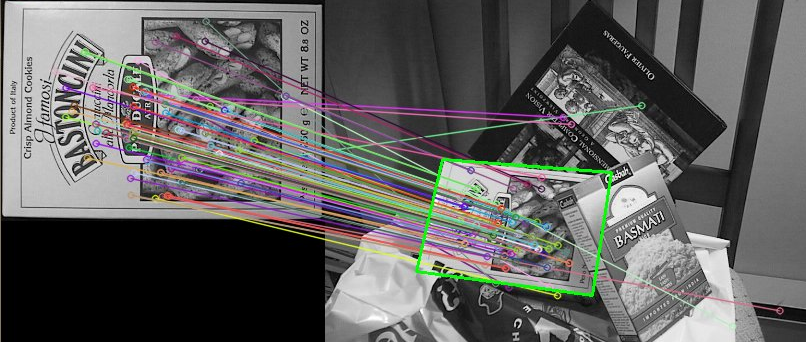
\includegraphics[width=0.8\textwidth]{img/rev_features2d_detection}
  \caption{Wykorzystanie framework-a cech 2d do wykrywania obiektów}
  \label{fig:rev_features2d_detection}
\end{figure}

Powyższy przykład pokazuje jak trudno zachować podział na wykrywanie
i~rozpoznawanie. Rysunek \ref{fig:rev_features2d_detection}
przedstawia sytuację, w~której wykrycie obiektu jest równoznaczne
z~jego rozpoznaniem.
Algorytm wylicza zestaw cech dla konkretnej okładki, po czym dla każdego
obrazu (w~przypadku pracy w~czasie rzeczywistym) wyliczany
jest dużo większy zestaw cech klatki. Jeżeli znaleziony zostanie
odpowiednio duży podzbiór cech podobnych na obu obrazach to wiadomo,
że obiekt znajduje się w~kadrze.
Dodatkowo, na podstawie ułożenia pasujących cech, możliwe jest
wyznaczenie jego zniekształcenia geometrycznego. W~kontekście wprowadzonego
podziału jest to raczej przykład lokalizacji poszczególnych instancji danej
klasy obiektów, niż wykrywanie obiektów klasy w~ogóle.
Poważnym
ograniczeniem jest wymóg posiadania dużej ilości szczegółów przez 
poszukiwany
obiekt, a~także wysoka rozdzielczość klatek, w~obrębie których odbywa się
poszukiwanie. Złożoność obliczeniowa, a~co za tym idzie czas przeszukiwania
poszczególnych klatek sprawiają, że metoda ta jest mało atrakcyjna w~kontekście
postawionego zadania.

Biblioteka OpenCV, w~omawianym jej fragmencie posiada znacznie
większą niż wspomniana funkcjonalność.
Ze względu na mnogość zaimplementowanych algorytmów - których opis
wykracza poza zakres tego opracowania - istnieje ogromna ilość
zastosowań wspomnianego frameworka. Jednym z~nich jest na przykład
detekcja obszarów
reprezentujących tekst w~scenach naturalnych. W~tym celu
można wykorzystać implementację algorytmu MSER - (\textit{ang. Most
Stable Extreme Regions}) \cite{OCV:MSER}.

\subsection{Open TLD - detekcja i~identyfikacja}

Kolejnym algorytmem łączącym w~sobie funkcje wykrywania
i~rozpoznawania obiektów jest algorytm opracowany przez
Zdenka Kalala \cite{DBLP:journals/pami/KalalMM12} - TLD (\textit{ang.
Track Learn Detect}).

Głównym zadaniem jakie rozwiązuje omawiany algorytm jest śledzenie obiektów.
Pewnym ograniczeniem jest potrzeba pierwszego oznaczenia interesującego
obiektu w~sekwencji obrazów tak aby możliwe było podjęcie pracy.
W~trakcie śledzenia tak oznaczonego obiektu odbywa się uczenie (doskonalenie)
detektora. O~ile sam etap śledzenia nie wykorzystuje detektora, to jest on
niezwykle istotny przy wznowieniu śledzenia po zniknięciu obiektu z~kadru.
Algorytm charakteryzuje się wysoką wydajnością i~zadziwiającą skutecznością.
Co prawda wyniki naocznych eksperymentów i~zamieszczonych przez autorów filmów
demonstracyjnych wyglądają efektownie, jednak bez narzędzi do automatycznego
mierzenia skuteczności trudno stwierdzić jaką klasę niezawodności 
i~skuteczności prezentuje omawiane rozwiązanie.

Kolejną kwestią jest obecność gotowych implementacji.
Dostępna jest co prawda wersja napisana w~języku C/C++ oraz MatLabie.
Niestety brak implementacji w~pakiecie OpenCV lub
innej gotowej wersji dostępnej na system Android jest kolejnym
argumentem przeciwko wykorzystywaniu TLD jako elementu
programu odczytującego numer autobusu na urządzeniu z~systemem Android.
Wymagająca analiza i~naniesienie
niezbędnych modyfikacji,
choć kształcące mogą nie przyczynić się do osiągnięcia zamierzonego celu.

Istnieje także przypuszczenie, że pozostawienie algorytmu w~trybie uczenia,
ze względu na rosnącą liczbę pozytywnych i~negatywnych obiektów w~bazie,
może powodować powolny spadek jego wydajności. Jest to jednak teza 
wymagająca przeprowadzenia rzetelnych testów, które ze względu
na nie wykorzystanie algorytmu w~rozwiązaniu końcowym nie zostały
wykonane.

\section{Rozpoznawanie obiektów - identyfikacja}

Drugim terminem poza detekcją, jest rozpoznawanie obiektów. Algorytm
odpowiedzialny za 
identyfikację najczęściej przyjmuje na wejściu obrazy stałych rozmiarów
\footnote{Co prawda nie jest to wymagane, jednak znacznie ułatwia 
wyliczenie wektora cech przypisanego do każdego zdjęcia, który to 
wektor dla większości popularnych implementacji musi być stałej 
długości.}.
Jego zadaniem jest zwrócenie
tekstu określającego typ, rodzaj lub po prostu nazwę danego obiektu.
Przykładem zastosowania może być odczytanie wykrytych liter,
cyfr, przypisanie twarzy do właścicieli lub zwrócenie marki wykrytego
samochodu.

Ze względu na specyfikę zagadnienia, gotowych implementacji algorytmów
identyfikacji jest niewiele lub sprawdzają się one w~obrębie
ściśle określonego zagadnienia. Niektóre z~przytoczonych w~poprzednim
podrozdziale przykładów mogą równie dobrze służyć jako identyfikatory
obiektów. Algorytm OpenTLD skutecznie rozróżnia twarze, gesty oraz
poszczególne instancje obiektów różnych klas.

Klasycznym podejściem do identyfikacji jest uczenie maszynowe. Na
wejściu podawany jest zbiór reprezentantów poszczególnych klas
z~przypisanymi do nich oczekiwanymi rezultatami. Rozwiązanie
sprawdza się przy rozpoznawaniu znaków drukowanych o~wysokim
kontraście i~w~wysokiej rozdzielczości. Utrudnieniem jest w~tym
przypadku znalezienie odpowiedniego przekształcenia obrazu
wejściowego na wektor cech, który jest właściwym 
parametrem wejściowym omawianej grupy algorytmów. W~skrajnych przypadkach
(np. wspomniane binarne obrazy reprezentujące znaki odpowiednio 
przycięte i~o~stałych rozmiarach) wektor może składać się 
z~wartości poszczególnych pikseli obrazu. W~sytuacjach bardziej 
skomplikowanych, niezbędne jest wstępne przetworzenie obrazu i/lub 
wykorzystanie przekształceń jak na przykład histogramy sum wartości
pikseli w~poszczególnych kolumnach lub wierszach, czy wspomniany
już wcześniej HOG (\textit{ang. Histogram of Oriented Gradients}).

Korzystając z~biblioteki
OpenCV \ można wybrać następujące metody:

\begin{itemize}
    \item model statystyczny,
    \item normalny klasyfikator bayesowski,
    \item k-najbliższych-sąsiadów,
    \item SVM,
    \item drzewa losowe,
    \item drzewa decyzyjne,
    \item sieci neuronowe,
    \item inne.
\end{itemize}

Częścią wspólną przedstawionych metod są fazy
fazy uczenia i~rozpoznawania, w~bibliotece
OpenCV reprezentowane przez funkcje \verb|train|, oraz \verb|predict|.

Niestety wybór metody obliczania wektora cech dla obrazów
pozostaje w~gestii programisty.
Można użyć deskryptorów cech
SIFT, SURF, BRIEF, HOG itp. W~skrajnie laboratoryjnych warunkach, tak
jak w~odczytywaniu znaków czarno-białych, można porównywać poszczególne
piksele. Jeżeli jednak tekst
jest ulokowany w~tak zwanej scenie naturalnej -
szyld, reklama, bilbord itp. - różnice w~czcionkach, refleksy
i~zniekształcenia uniemożliwiają wykorzystanie tak trywialnej metody.

Zagadnienie jest na tyle ważne i~jednocześnie skomplikowane, że
powstał plebiscyt, którego zadaniem jest wyłonienie najlepszego
algorytmu odczytującego teksty ze scen naturalnych. Odbywa się
on co dwa lata, a~ostatnia edycja miała miejsce w~roku 2013.
Zwycięzcy konkursu ICDAR2013 w~dziedzinie odczytywania tekstu ze
zdjęć, do rozpoznawania poszczególnych znaków wykorzystali sieci neuronowe.
Podobnie było w~przypadku algorytmu odczytującego numery domów na potrzeby
geolokalizacji w~usłudze Google:StreetView. Ostatecznie zadanie
odczytywania numerów/tekstów ze zdjęć jest zadaniem najtrudniejszym
z~dotąd omawianych.

\begin{figure}[h!]
    \centering
    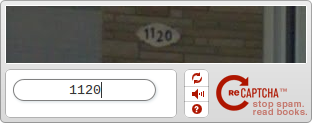
\includegraphics[width=0.8\textwidth]{img/rev_captcha_street_view}
    \caption{Przykładowa captcha z prawdopodobnym numerem domu}
    \label{fig:google_street_view_captcha}
\end{figure}

O~skali złożoności problemu może świadczyć fakt, iż
opracowany przez Google algorytm wymaga wspomagania w~postaci
ręcznej interwencji
operatorów. Proces został na wpół zautomatyzowany, 
poprzez wykorzystanie internautów do ręcznego
przepisania numeru domu np. podczas logowani, rejestracji lub innej
czynności wymagającej zabezpieczenia przed szkodliwą działalnością
automatów - rysunek \ref{fig:google_street_view_captcha}.



\chapter{Przygotowanie środowiska - automatyzacja}

Rozpoznanie numeru autobusu, ze względu na niewielką moc obliczeniową
urządzeń mobilnych, wymagć będzie zastosowania algorytmu składającego się
z~co najmniej kilku kroków. Kolejne stopnie kaskady uszeregowane powinny 
być w~taki sposób, aby operując na dużych zbiorach danych - np.: pełne 
klatki z~kamery w~wysokich rozdzielczościach - używać algorytmów o~możliwie
najniższej złożoności obliczeniowej celem zawężenia pola poszukiwań.
Postępująca segmentacja obrazu miałaby umożliwić rozpoznanie
numeru autobusu w~czasie rzeczywistym, nie zależnie od klasy urządzenia.

Biorąc pod uwagę powyższe wymagania pierwszym krokiem (założenie robocze)
algorytmu powinna być segmentacja obrazu poprzez wykorzystanie kaskadowego
detektora haara lub LBP (powinny być opisane w~części teoretycznej).
Ze względu na różnice pomiędzy tymi dwoma detektorami pierwszym
doświadczeniem wykonanym na potrzeby tego opracowania będzie porównanie
ich wydajności i~dokładności. 

Sam proces uczenia detektorów jest jednak przedsięwzięciem żmudnym.
Dodatkowo wymaga on dużych zbiorów danych uczących oraz zbioru testowego.
W~następnych podrozdziałach przedstawione zostaną narzędzia których
zadaniem będzie maksymalna automatyzacja i~optymalizacja procesu uczenia
oraz weryfikacji zarówno skuteczności jak i~wydajności uzyskanych wersji
detektorów.

Oczywiście w~dalszych podrozdziałach opisane zostaną kolejne robocze
kroki algorytmu, a~także narzędzia służące w~ich przygotowaniu oraz 
weryfikacji.

Celem tego rozdziału jest więc udokumentowanie doświadczeń przeprowadzonych
na drodze do osiągnięcia optymalnego algorytmu rozpoznawania numeru
autobusu.

\section{Wspomaganie pobierania filmów z serwisu YouTube}

Pewnego rodzaju rozgrzewką było przygotowanie wtyczki do przeglądarki 
Firefox ułatwiającej pobieranie i wstępne katalogowanie filmów
udostępnianych za pośrednictwem serwisu YouTube.

Założenia oraz oczekiwania funkcjonalne wobec omawianego narzędzia były 
następujące:

\begin{enumerate}
    \item Wizualizacja stanu w~jakim znajduje się oglądany film - 
        możliwe są dwa stany:
    \begin{itemize}
        \item co najmniej jedna wersja filmu została już pobrana,
        \item film nie został pobrany w~żadnej wersji.
    \end{itemize}
    \item Możliwość pobrania wybranej wersji filmu w~odległości maksymalnie
        dwuch kliknięć licząc od poziomu przeglądania filmów w~serwisie,
    \item Tworzenie pliku CSV (\textit{ang. Comma Separated Value})
        z~danymi pobranych filmów, celem identyfikacji już pobranych
        pozycji. Plik powinien być tak skonstruowany aby można go było
        również wykorzystać do odtworzenia bazy filmów na dysku. W~razie
        awarii lub chęci przeprowadzenia całego procesu uczenia od
        początku.
\end{enumerate}

\subsection{Pierwsza wersja wtyczki - stan}

Przedstawienie stanu aktualnie oglądanego filmu odbywa się poprzez
kolor dodatkowej ikony wkomponowanej w~lewe pionowe menu, zaraz obok
wyświetlanego filmu.

\begin{figure}[h!]
    \caption{Przycisk rozwijanego menu, oraz wskaźnik stanu}
    \centering
    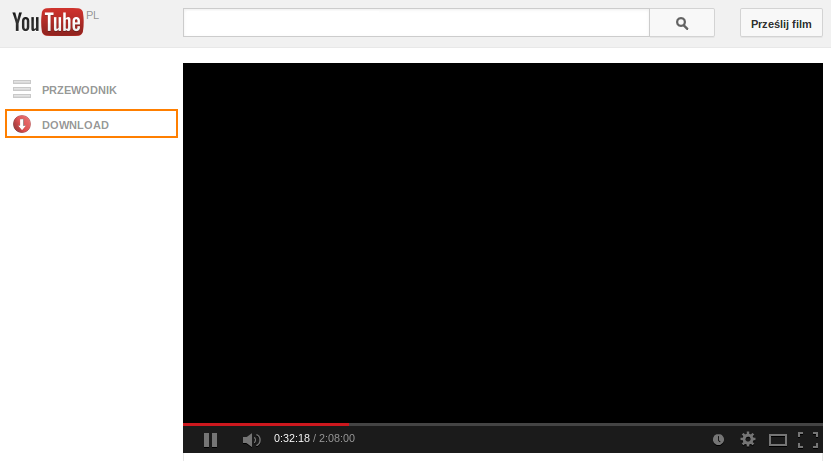
\includegraphics[width=0.9\textwidth]{img/env_yt_dwn_indicator}
\end{figure}

Kolor czerwony wskazuje, że oglądany film nie został jeszcze pobrany.
Ikona z~pustą strzałką w~środku w~kolorze zielonym sygnalizuje obecność
oglądanej pozycji w~wyżej wymienionym pliku rozdzielanym przecinkami
(pkt. 3).

Postępy w~pracach nad pierwszą wersją wtyczki doprowadziły do wypełnienia
założeń funkcjonalnych przez ostatnią wersję programu. Koncepcja wkomponowania
menu w~treść strony, oraz funkcjonalność pobierania filmów okazały się
na tyle problematyczne i~trudno zarządzalne, że powstała druga wersja programu
o~znacznie ograniczonej funkcjonalności.

\subsection{Druga wersja wtyczki - funkcjonalność}

Funkcjonalność drugiej wersji programu została ograniczona do minimum. Faktycznie
ograniczała się ona do oznaczania wybranego filmu wraz z~jego wersją, oraz
eksportu tak utworzonych wpisów do pliku - id filmu oraz numer identyfikacyjny wersji.

Przepływ sterowania dla drugiej wersji programu został przedstawiony na poniższym
diagramie. Funkcja implementująca pokazany algorytm jest wywoływana za każdym razem
gdy zmieni się wartość url-a w~aktywnej karcie przeglądarki lub kliknięty zostanie
któryś z~przycisków w stanach ,,żółtym'' lub ,,zielonym''.

\begin{figure}[h!]
    \caption{Algorytm aktualizacji stanu wtyczki w wersji drugiej}
    \centering
    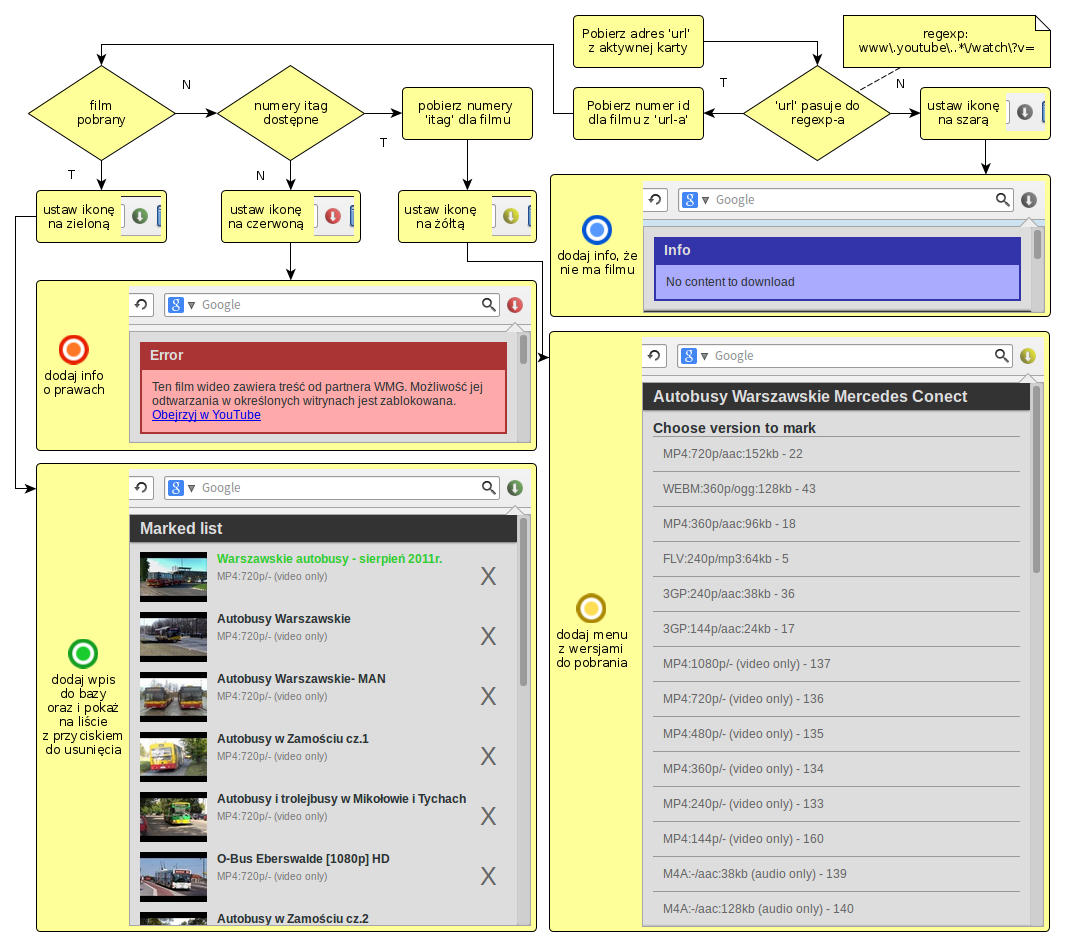
\includegraphics[width=0.9\textwidth]{img/env_yt_marker}
\end{figure}

Niestety program pierwszy program ,,pomocniczy'' okazał się narzędziem nie adekwatnym
(zbyt skomplikowanym i~pracochłonnym) do postawionego mu zadania. Okazało się, że
filmów zawierających fronty autobusów jest znacznie mniej niż mogło by się wydawać.

Po znalezieniu 14 pozycji zawartość serwisu (odnośnie frontów autobusów) nagle się
wyczerpała. Ostatecznie wielotygodniowe (dokładnie dwu) prace nad wtyczką do programu 
Firefox zaowocowały bazą czternastu pozycji w~formie pliku CSV zawierającego dwie
kolumny:

\begin{itemize}
    \item id filmu, np.: 75Dz6s7S-Tg;
    \item itag reprezentujący wybraną wersję, np.: 136
\end{itemize}

W~naszym przypadku wszystkie filmy zostały ,,oznaczone'' w~wersji 136, czyli
zawierającej tylko obraz, oraz będącej w~rozdzielczośći HD (720p).

Ostatecznie owoc pracy przedstawiony jest poniżej.

\lstinputlisting{../data/description_files/marked_for_download/yt_marked_01.csv}

Co niestety o~wiele szybciej, prościej, wydajniej, taniej i~krótko mówiąc lepiej można
by wykonać bez implementowania żadnych narzędzi. Jedyne co pozostało to zdobyta wiedza
na temat: javascript, css, html, firefox: xul, addon-sdk, cfx. 

Kolejne narzędzia ,,pomocnicze'' implementowane będą z~większą ostrożnością i~po
dłuższym przeanalizowaniu zagadnienia poddawanego automatyzacji.

\section{Tworzenie zbioru wejściowego do narzędzia train\_cascade}

Mając plik z~identyfikatorami filmów na serwisie YouTube wszystkie duże objętościowo
dane potrzebne przy tworzeniu wsadu od narzędzia uczącego można było zostawić
w~ich pierwotnym położeniu. Tworząc narzędzie wspomagające oznaczanie frontów
wzbogacono je o~możliwość odtworzenia osiągniętego stanu w~oparciu o~pliki konfiguracyjne.
Dodana funkcjonalność i~systematyczne wypychanie danych do zewnętrznego repozytorium
umożliwiły niezakłuconą kontynuację prac po awarii i~utracie lokalnej kopii.

Interfejsem narzędzia odpowiedzialnego za przygotowanie danych uczących był skrypt
napisany w~języku python:

\lstinputlisting{data/autocascader.txt}

\subsubsection{Odtwarzanie środowiska po awarii}

Pierwszym krokiem było pobranie plików wideo. W~tym celu należało wywołać skrypt
z~parametrem -d.

Po drobnych poprawkach (utworzeniu katalogu na pobrane pliki, którego nie było
w~repozytorium) i~popbraniu wymaganych zależności proces poprawnie pobrał
11 (jedenaście) zdefiniowanych w~pliku konfiguracyjnym pozycji.

Ostatecznie wywołanie skryptu z~parametrem -e poprawnie wyłuskało klatki
z~pobranych plików, które zostały zapisane w~postaci obrazów w~katalogach
odpowiadających ich przeznaczeniu:

\begin{itemize}
\item front - pliki reprezentujące generyczne fronty autobusów,
\item solaris - pliki reprezentujące fronty autobusów solaris (dla porównania),
\item background - pliki tła - nie zawierające wystąpień żadnych frontów.
\end{itemize}



\chapter{Eksperymenty}

\section{Pierwszy krok kaskady - lokalizacja frontu autobusu}

\subsection{Zbiór danych uczących i testowych}

Pierwszą partią danych ucząco-testowych było 11 zestawów obrazów
przygotowanych z~uprzednio pobranych filmów z~serwisu YouTube.

Każdy zestaw składał się z co najmniej dwuch zbiorów obrazów 
reprezentujących oznaczone fronty autobusów oraz obrazy tła
(ang. background). Opcjonalnym zbiorem był zestaw oznaczonych 
frontów autobusów typu solaris. Osobny zestaw frontów miał na celu
porównanie skuteczności detektorów przygotowanych tylko przy pomocy
pojedynczego typu obiektu oraz tych do przygotowania których użyto
obiektów znacząco od siebie różnych.

\subsubsection{Zbiór jJ9ixBfVR5k}

\begin{figure}[!h]
    \centering
    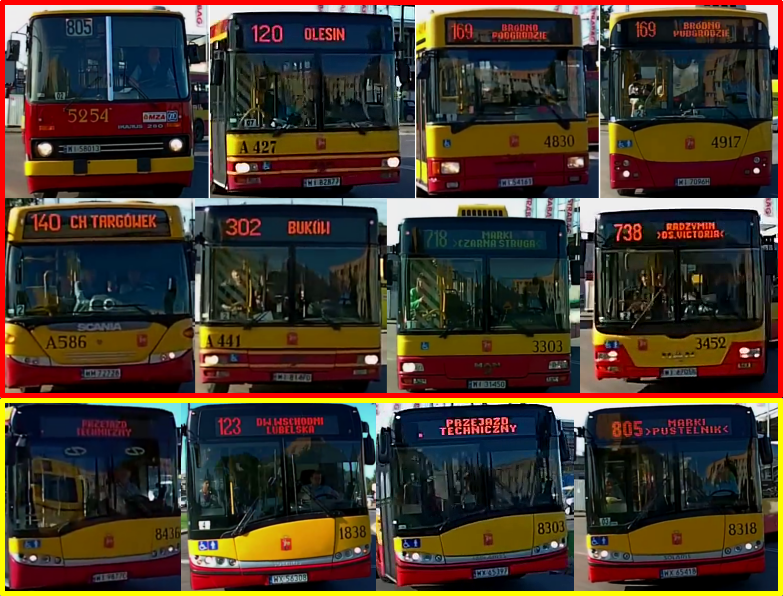
\includegraphics[width=0.9\textwidth]{img/exp_trainig_data_jJ9}
    \caption{Typy autobusów zawarte w zbiorze jJ9ixBfVR5k}
    \label{fig:jJ9ixBfVR5k_types}
\end{figure}

\begin{table}[!h]
    \centering
    \begin{tabular}{c|c|c}
        Front   & Solaris   & Background \\
        2587    & 222       & 2239
    \end{tabular}
    \caption{Liczebność zbioru jJ9ixBfVR5k}
    \label{tab:jJ9ixBfVR5k_count}
\end{table}

\subsubsection{Zbiór vYqZ4-tH4M0}

\begin{figure}[!h]
    \centering
    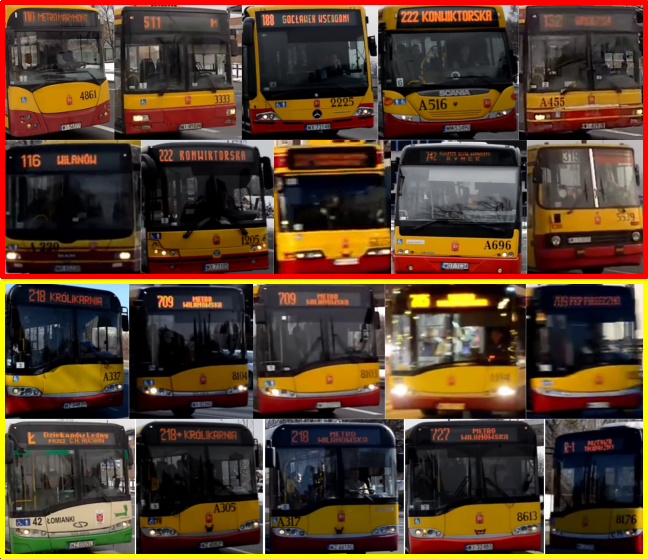
\includegraphics[width=0.9\textwidth]{img/exp_trainig_data_vYq}
    \caption{Typy autobusów zawarte w zbiorze vYqZ4-tH4M0}
    \label{fig:vYqZ4-tH4M0_types}
\end{figure}

\begin{table}[!h]
    \centering
    \begin{tabular}{c|c|c}
        Front   & Solaris   & Background \\
        2587    & 222       & 2239
    \end{tabular}
    \caption{Liczebność zbioru vYqZ4-tH4M0}
    \label{tab:vYqZ4-tH4M0_count}
\end{table}

Pierwsza iteracja uczenia detektorów miała na celu przetestowanie
opcji jakie można zadać narzędziu uczącemu - opencv\_traincascade.

Za zbiór testowy posłużył zestaw oznaczonych zdjęć oraz zdjęć tła
przygotowany dla filmu o id jJ9ixBfVR5k:
\begin{itemize}
\item oznaczone fronty: 2587,
\item oznaczone fronty typu solaris: 222,
\item obrazy tła: 2239.
\end{itemize}

Pierwszy test miał za zadanie wyłonić najefektywniejszą metodę, do dalszych
eksperymentów. Narzędzie dostarczone wraz z~pakietem OpenCV - wspomniany
już opencv\_traincascade - umożliwia ,,wyszkolenie'' trzech rodzai
detektorów:

\begin{itemize}
    \item detektor wykorzystujący tzw. cechy Harra - wartość 
        domyślna (HAAR),
    \item detektor LBP,
    \item detektor HOG.
\end{itemize}

\begin{table}[!h]
    \centering
    \begin{tabular}{r|c|c|c|l}
        & HAAR         & LBP        & HOG              &       \\
        \hline
Solaris & 151  (43\%)  & 81  (23\%) & 61 (17\%)        & /346  \\
Różne   & 1051 (35\%)  & 748 (25\%) & 712 (24\%)       & /2925 \\
Tło     & 635  (11\%)  & 386 (6\%)  & 447 (7\%)        & /5588 \\
    \end{tabular}
    \caption{Porównanie skuteczności detektorów typu HAAR, LBP i HOG.}
    \label{tab:haar_lbp_hog_comparison}
\end{table}

Czas uczenia poszczególnych detektorów różnił się dość znacząco. Proces
uczenia detektora Haar-a trwał ponad 6 godzin, podczas gdy dla detektorów
BLP oraz HOG były to odpowiednio 42 minuty oraz 3 godziny i 10 minut.



\bibliographystyle{plain}
\bibliography{src/bibliography}

\end{document}
